\section{Complex Nodes}

\tikzstyle{place}=[circle,draw=blue!50,fill=blue!20,thick, inner sep=0pt,minimum size=6mm]
\tikzstyle{transition}=[rectangle,draw=black!50,fill=black!20,thick, inner sep=0pt,minimum size=4mm]


\begin{frame}{Complex Nodes}
\begin{figure}
    \centering
    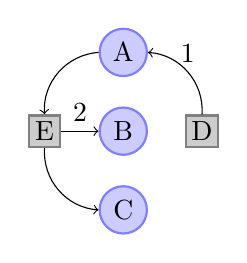
\begin{tikzpicture}
\node[place] (waiting) {A};
\node[place] (critical) [below of=waiting] {B};
\node[place] (semaphore) [below of=critical] {C};
\node[transition] (leave critical) [right of=critical] {D}
edge [-> , bend right = 45] node[above] {1} (waiting);
\node[transition] (enter critical) [left of=critical] {E}
edge [->] node[above] {2} (critical)
edge [<-,bend left=45] (waiting)
edge [->,bend right=45] (semaphore);
\end{tikzpicture}
    \caption{Flow}
\end{figure}
\end{frame}



\begin{frame}{Complex Node 2}

\begin{figure}
    \centering
    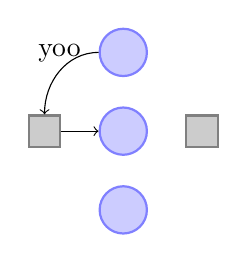
\begin{tikzpicture}
\node[place] (waiting) {};
\node[place] (critical) [below of=waiting] {};
\node[place] (semaphore) [below of=critical] {};
\node[transition] (leave critical) [right of=critical] {};
\node[transition] (enter critical) [left of=critical] {};
\draw [->] (enter critical) -- (critical);
\draw [->] (waiting) to [in = 90, out = 180] node[anchor = south] {yoo} (enter critical);
\end{tikzpicture}
    \caption{Caption}
\end{figure}
    
\end{frame}